% Chapter 1

\chapter{Recherche d'image par le contenu} % Main chapter title

%\label{Chapter1} % For referencing the chapter elsewhere, use \ref{Chapter1} 

%\lhead{Chapter 1. \emph{Recherche d'image par le contenue}} % This is for the header on each page - perhaps a shortened title

%----------------------------------------------------------------------------------------

\section{Introduction}

	De nos jours, un grand nombre d'images est généré et transmis sous format numérique sur Internet, et il existe une variété d'outils permettant d'accéder à ces images numériques. Cependant, lors de la recherche d'une image à partir d'Internet en utilisant un moteur de recherche d'images (par exemple: Google [Figure 1.1]), les résultats récupérés ne répondent pas forcément au besoin de l'utilisateur. En effet, les images sont retrouvées en se basant sur les métadonnées associées comme les mots clés, les titres, etc.
	
	
\begin{figure}[H]
	\centering
		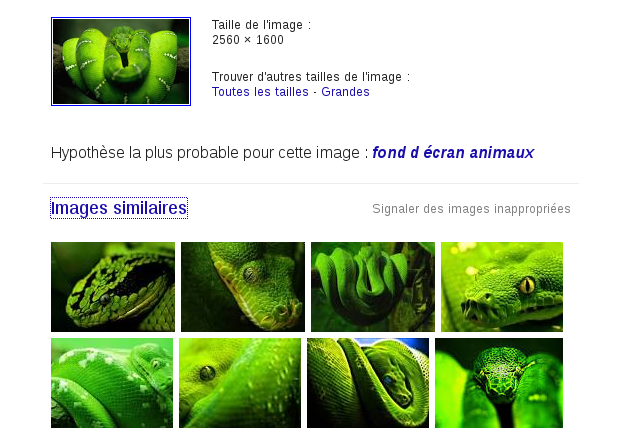
\includegraphics[width=3.5in]{Figures/googleImage2.png}
	\caption[An Electron]{Recherche d'image de Google.}
	\label{fig:Electron}
\end{figure}

	La recherche d'image par texte (Text Based Image Rertieval - TBIR) [Figure 1.2] dépend de la qualité des annotations d'une image qui doivent couvrir tous les termes désirés, cette tâche peut être donc difficile, coûteuse ou même encore infaisable quand la collection d'images est trop large.
	
\begin{figure}[H]
	\centering
		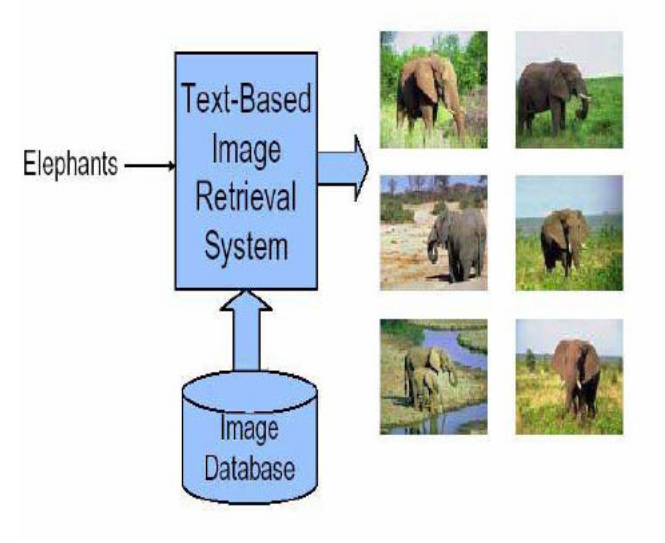
\includegraphics[width=3in]{Figures/textBasedIR.png}
	\caption[An Electron]{Recherche d'image par texte. [Shr et al. 13]}
	\label{fig:Electron}
\end{figure}
	
	La recherche d'image par le contenu (Content Based Image Retrieval - CBIR) [Figure 1.3] propose des techniques pour éviter l'utilisation des descriptions textuelles, et permet de récupérer les images pertinentes à partir d'une grande collection de base d'image. Les techniques de récupération d'images se basent sur certaines caractéristiques récupérées du contenu de l'image, comme la texture, la couleur, la forme, etc.

\begin{figure}[H]
	\centering
		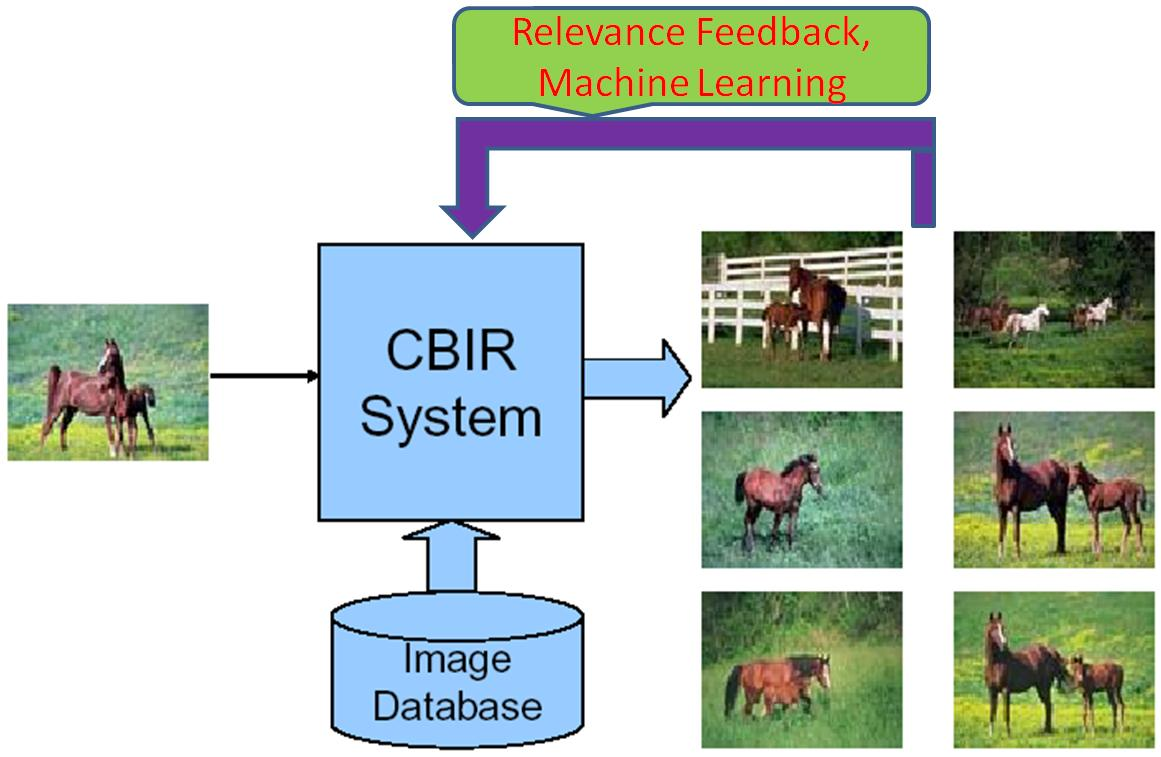
\includegraphics[width=3.5in]{Figures/cbir.JPG}
	\caption[An Electron]{Recherche d'image par le contenu. [Shr et al. 13]}
	\label{fig:Electron}
\end{figure}


	Pour réaliser un système de recherche d'image par le contenu, des techniques basées sur le contenu des images ont été développées, et qui font appel à deux domaines de recherches:

\textbf{Gestion de base de données:} plus le nombre d'images dans une base est grand et plus il est nécessaire d'optimiser les méthodes de stockages, l'indexation multidimensionnelle des images et le temps de réponse à une requête.

\textbf{Vision artificielle:} ce domaine propose des techniques et approches pour la représentation et extraction des caractéristiques du contenu des images.


\section{La conception d'un système CBIR}

	Les systèmes de recherche d'images par le contenu sont généralement basés sur des caractéristiques ou descripteurs d'images, par exemple:
	
\begin{itemize}

\item \textbf{Descripteur  de couleur:} grâce à leurs représentations compactes et de faible complexité, la comparaison directe des histogrammes de couleur est communément utilisée.
\item \textbf{Descripteur de forme:} descripteur de Fourier et moment invariant.
\item \textbf{Descripteur de texture:} ces techniques permettent de donner une description des textures sous forme de mesures d'énergie, de contraste, d'homogénéité, etc. comme les matrices de co-occurence (GLCM)[Har 79], ou bien sous forme d'histogramme comme le Local Binary Pattern (LBP) [Oja et al. 02].
\item \textbf{Descripteur local:}  l'information numérique est dérivée de l'analyse locale d'une image caractérisant son contenu visuel de la façon la plus indépendante possible de l'échelle, du cadrage, de l'angle d'observation et de l'exposition. C'est des descripteurs assez récents tel que Scale-invariant feature transform (SIFT) [Low 99].

\end{itemize}

\section{Calcul de similarité}

	Généralement, des fonction rigides de calcul de distance comme la distance euclidienne ou la similarité basée sur le cosinus sont utilisées pour la recherche de ressemblance entre les caractéristiques extraites.

	Par-contre, ces fonctions de calcul de distance et de similarité ne sont pas toujours optimales pour la tâche complexe de recherche d'images par le contenu, cela est dû au problème du fossé sémantique (Semantic Gap) entre les caractéristiques bas niveau extraites par l'ordinateur, et le haut niveau de perception humaine.

	Récemment, de grands efforts ont été fournis dans la recherche de différentes méthodes de calcul de similarité en utilisant les techniques de l'apprentissage automatique. Parmi ces dernières, des travaux se sont concentrés sur l'apprentissage de hachage. Des propositions ont été faites pour des méthodes d'apprentissage de mappage de données de hautes dimensions vers des codes binaires qui préservent la similarité sémantique. [Sin et al. 15]

\section{Problème du faussé sémantique}

	Parmi les problèmes  les plus difficiles qui font face à la recherche d'image par le contenu, nous trouvons le fossé sémantique. Il est défini comme la différence entre la faible niveau de représentation de l'information (y compris, mais pas seulement des images) dans l'ordinateur et la sémantique de haut niveau derrière elle (en d'autres mots, le sens qu'il doit représenter).
	
	Récemment, de nouvelles approches pour résoudre ce problème, consistent en appliquant des techniques d'apprentissage automatique pour permettre à l'ordinateur de construire sa propre représentation hiérarchique d'une image, au lieu de calculer les caractéristiques manuellement.


\section{Types de CBIR [Shr et al. 13]}

	Nous allons présenter quatre exemples d'approches conceptuelles différentes qui ont été développées pour les systèmes de recherche d'image par le contenu:

\subsection{Basée-région}

	Netra [Ma et al. 99] et Blobworld [Car et al. 99] sont deux anciens systèmes de recherche d'images par le contenu basées région. Au moment de la recherche, le système fourni à l'utilisateur des régions segmentées de l'image requête, et il lui demande d'attribuer plusieurs propriétés, tel que les régions à mettre en correspondance, les caractéristiques des régions ou même le poids des différentes caractéristiques.


\subsection{Basée-objets}
	
	Les systèmes de récupération d'image basées sur les objets retrouvent des images à partir d'une base de données en se basant sur l'apparence des objets physiques dans ces images. Ces objets peuvent être des éléphants, des panneaux d'arrêt, des hélicoptères, des bâtiments, des visages ou tout autre objet que l'utilisateur souhaite trouver. Une façon courante pour rechercher des objets dans les images est d'abord de segmenter toutes les images dans la base de données puis de comparer chaque région segmentée avec une région de l'image requête présentée par l'utilisateur. Ces systèmes de récupération d'image donnent de très bons résultats pour les images qui contiennent des objets qui peuvent être facilement séparés de l'arrière-plan, et qui ont des couleurs distinctives ou même des textures.

\subsection{Basée-exemples}

	Appelée aussi recherche d'image par le contenu basée-requête, nous nous intéresserons dans nos approches à cette catégorie qui sera détaillée dans le troisième chapitre. Les utilisateurs donnent une image requête, ou une partie d'une image, le système l'utilisera comme base pour sa recherche. Il devra trouver à l'aide de caractéristiques extraites du contenu de l'image, toute les images semblables qui partagent ce même contenu.


\subsection{Basée-Feedback}
	Pour rechercher une image, le système affiche à l'utilisateur un échantillon de photos et demande à l'utilisateur des les classer. En utilisant ce classement, le système ré-exécute les requêtes et répète cela jusqu'à ce que la bonne image soit trouvée.

\section{Systèmes de recherche d'images existants}

	Les systèmes de recherche d'image par le contenu ont été utilisés dans un grand nombre d'applications telles que: le diagnostic médical [Figure 1.4], les archives photographiques, l'identification des empreintes digitales et la reconnaissance faciale.


\begin{figure}[H]
	\centering
		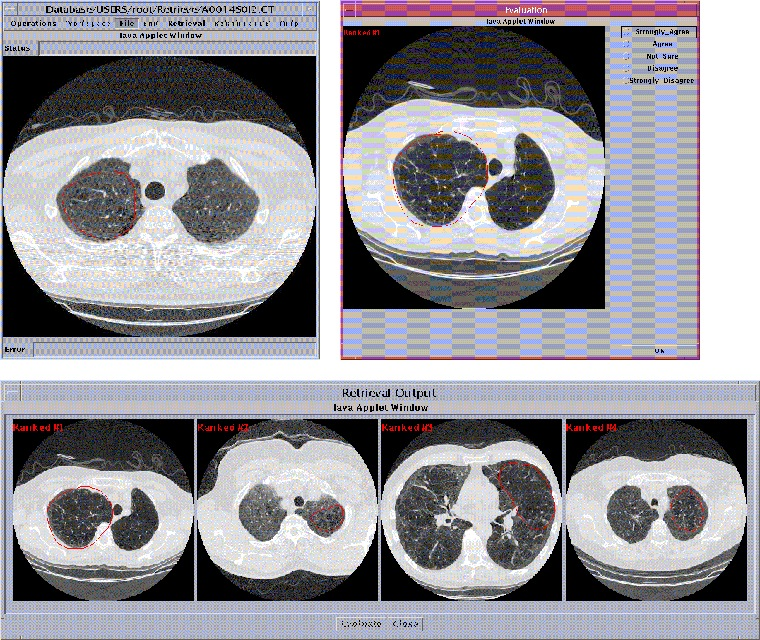
\includegraphics[width=2.5in]{Figures/cbirMedic.jpg}
	\caption[An Electron]{Application Médicale. [Yod 08]}
	\label{fig:Electron}
\end{figure}

	Nous allons maintenant présenter quelques systèmes connus de recherche d'image par le contenu:

\subsection*{QBIC}
	Query By Image Content (QBIC) [Nib et al. 93][Fli et al.95], signifie requête par contenu d'image, il est le premier système de recherche d'images par le contenu commercial. Il fournit des framework et des techniques de base pour de nombreux systèmes de récupération d'images. QBIC supporte les requêtes basée sur des exemples d'images, d'images construites par l'utilisateur, des dessins et modèles de couleur et de texture, etc. Les fonctions de couleur utilisées dans QBIC sont (R, G, B), (Y, i, q), ( L, a, b), MTM (transformée mathématique Munsell), et un histogramme de couleur à k-élément. Dans son nouveau système, la recherche de texte par mot-clé peut être combinée avec la recherche de similarité par contenu. La [Figure 1.5] montre une démo de QBIC.

\begin{figure}[H]
	\centering
		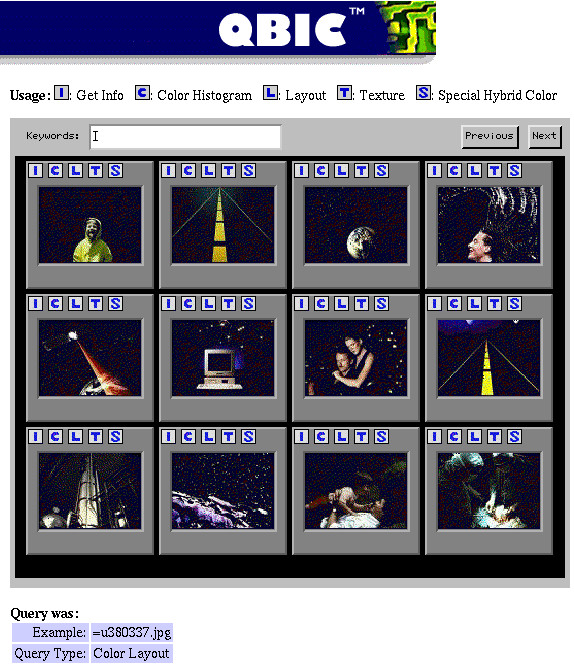
\includegraphics[width=3in]{Figures/qbic-demo.jpg}
	\caption[An Electron]{Interface de la démo de QBIC.}
	\label{fig:Electron}
\end{figure}

\subsection*{LIRE}
	LIRE [Lux et al. 08][Lux et al. 13] est une bibliothèque Java qui fournit un moyen simple permettant de rechercher des photos et des images en fonction de leurs caractéristiques de couleur et de texture. LIRE crée un index de Lucene des caractéristiques de l'image pour la récupération de son contenu. Elle est facile à utiliser, des méthodes pour rechercher l'index et les résultat sont fournies par LIRE.
	
	La bibliothèque LIRE et l'application de démo [Figure 1.6] ainsi que tous les fichiers sources de test et de développement sont disponibles sous la licence GNU GPL.

\begin{figure}[H]
	\centering
		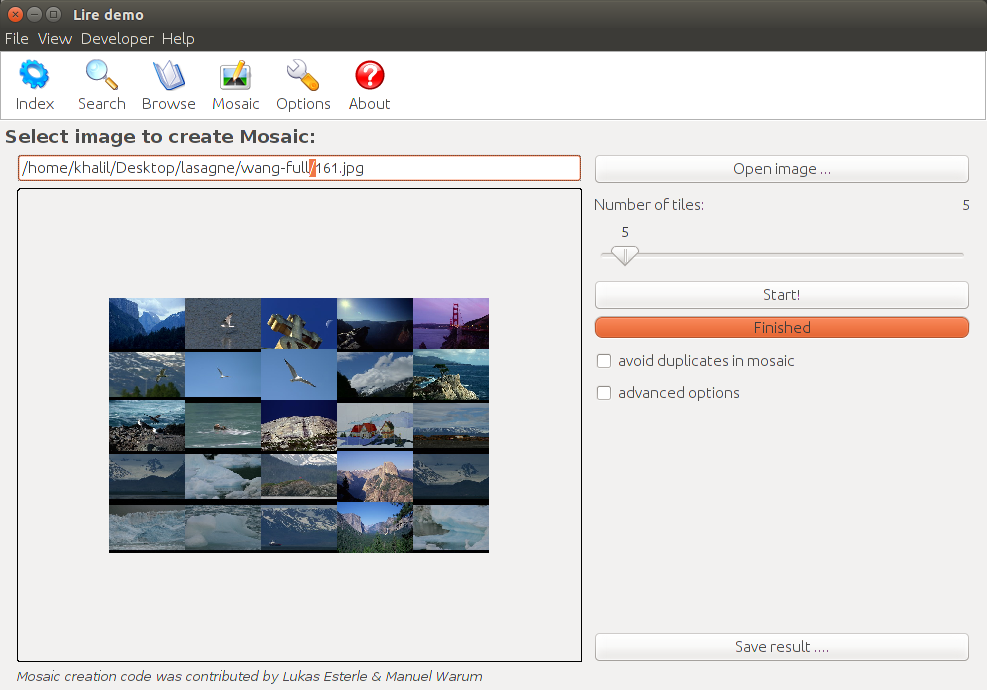
\includegraphics[width=4in]{Figures/lire-demo.png}
	\caption[An Electron]{Interface de la démo de LIRE.}
	\label{fig:Electron}
\end{figure}


\subsection*{FIRE}
	Flexible Image Retrieval Engine (FIRE) [Des et al. 08], c'est un système de recherche d'images par le contenu que Thomas Deselaers a developpé avec d'autres chercheurs de The Human Language Technology and Pattern Recognition Group de RWTH Aachen University.

L'objectif principal de FIRE est d'étudier différents descripteurs d'image et d'évaluer leur performance. FIRE a été développé en C ++ et Python et est destiné à être facilement extensible. Une démo est disponible comme le montre la figure suivante:


\begin{figure}[H]
	\centering
		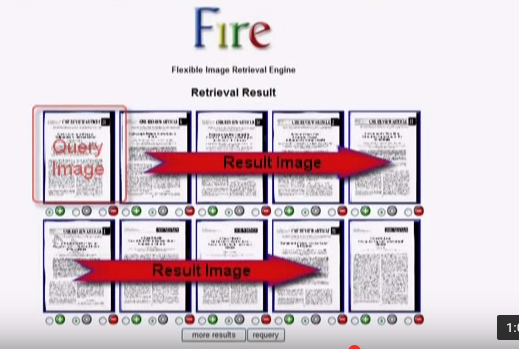
\includegraphics[width=5in]{Figures/fire-demo.png}
	\caption[An Electron]{Interface de la démo de FIRE.}
	\label{fig:Electron}
\end{figure}

\subsection*{DigiKam}
	DigiKam est un logiciel gratuit et open-source organisateur d'image et éditeur de tag écrit en C++, c'est aussi une application de gestion de photos étendue construite avec des bibliothèques de KDE. Il offre, en plus d'autres nombreuses fonctionnalités: les recherches inversées pour les images de la collection locale, la détection de doublons et la recherche floue par des dessins.

%D'autres projets comprennent:
%- The GNU Image-Finding Tool
%- Google Image Search
%- eBay Image Search

%Une liste plus exhaustive peut être trouvée dans ce article :

%$$https://en.wikipedia.org/wiki/List_of_CBIR_engines$$


\section{Conclusion}
	
	Dans ce chapitre nous avons fait une introduction sur les systèmes de recherche d'image par le contenu, puis nous avons ensuite présenté quelque types de CBIR dont la recherche d'image par le contenu basée-exemple 
sur laquelle notre implémentation se base. On a conclu ce chapitre par des exemples de systèmes connus de recherche d'image par le contenu.

	Nous allons présenter dans le prochain chapitre des technique d'apprentissage automatique et principalement d'apprentissage profond pour essayer de proposer des solutions au problème du fossé sémantique des images.